\section{Introduction}

Statistical methods for analyzing network data are becoming increasingly useful for studying phenomena ranging from online social behavior to protein  interactions \cite{Goldenberg2009}.
Recent work has expanded to include settings in which we observe events occurring between nodes over time (i.e., \emph{relational events}, as opposed to static edge structures or ongoing relationships), with the common goal of modeling interaction dynamics in terms of both endogenous mechanisms and exogenous covariates.  
A key concern in this regard is the ability to detect differential behavioral tendencies on the part of subsets of nodes, the dynamic analog of \emph{role structure} in classical network analysis \cite{Wasserman1994}.  

In the cross-sectional case, \emph{stochastic blockmodels} \cite{Nowicki2001, Kemp2006, Ishiguro2010, Rodriguez2011} have been proposed as a family of approaches that capture behavioral similarity by identifying subsets of nodes with similar patterns of ties to those in other sets.  While it is natural to apply these ideas directly to relational event data via blockmodeling of the time-marginalized rates of interaction among dyads (effectively treating the event structure as a valued graph), there are limits to what this approach can detect.  Consider, e.g., Figure~\ref{fig:introexample}.  In the top left panel, we depict the time-marginalized frequencies of simulated interactions between members of two groups (A and B), with darker cells indicating higher interaction frequencies.  As can be seen, a clear role structure is present, with members of each subgroup interacting at higher rates with co-members than out-group members; such a structure is easily detectable via conventional blockmodeling techniques.  By contrast, consider the interaction patterns shown in the top right panel.  Here, there is no systematic difference in marginal rates between the two groups, rendering them invisible under a standard blockmodeling approach.

There is, however, a difference to be detected.  The bottom panels of Figure~\ref{fig:introexample} show, for each respective simulation, parameters (as discussed in Section~\ref{sec:specification}) governing the tendency towards reciprocation for members of each group vis a vis communications coming from in- or out-group members.  For both simulated cases, the log-hazard for an event in which a member of group A or group B immediately responds to an incoming communication from an in-group member is increased by an increment of 2 (relative to a non-reciprocating event), and the log-hazard for an event in which a member of group B immediately responds to an incoming communication from a member of group A is increased by a corresponding increment of 0.5.  Groups A and B are thus distinctive in terms of their dynamic behavior, even in the absence of marginal differences in propensity to communicate.  A blockmodeling approach that classifies nodes based on shared dynamics (rather than merely shared marginal communication rates) can potentially identify such subtle distinctions; in this paper, we introduce such an approach.


%For example, a common aspect of human communication is \emph{reciprocity}: person A speaks to person B, then B has a higher propensity to speak to A.  
%Through an event-based analysis we can study how nodes vary in their tendencies to behave in this manner.  %the similarity --- and differences --- in the dynamics of nodes in the network. 
%This is particularly relevant when studying interactions among students in a classroom, where differences in conversational tendencies might be associated with covariates about the student or classroom, or based on unobserved groupings, and may have ramifications for education.
%In such contexts, a standard blockmodel only provides a means for studying the structure of marginal rates of communication, but not the shared tendencies in the dynamics of the sequence of events.

%When such .  One unifying idea is that the nodes of these networks are differentiated by rates of interacting with other parts of the network [TODO], where this variation in rates may be associated with some unobserved quantity, e.g. a covariate such as age or sex, or perhaps shared [TODO].
%Stochastic blockmodels \cite{Nowicki2001, Kemp, Ishiguro2010, Rodriguez} are a class of statistical models for static network data that employ latent variables to model this heterogeneity by .  Such techniques are readily applied to count data, [TODO: These let us study how shared behavior is associated with other covariates.]

%1) assuming each node in the network belongs to some block (or cluster) and 2) parameterizing the probability of a tie between members

%PS: much of this past work is for static network data. Do we want to make the observation here that we are thinking about blockmodels for *rate* data here in our discussion and in our example in figure 1 - if we don't some readers/reviewers might get a little confused. For example we could say that instead of a binomial model on edges we can think of a Poisson process yielding counts over time, where we can still think about blockmodels. 
%PS: also, we introduce the term "rates" above without really defining it, and then go on to talk about "mean rate" below. So I think we definitely need a sentence somewhere above that makes it clear we are talking about edges that instantaneously appear and disappear over time at some rate, rather than static edges.

%If we are interested in studying a network of events, there are other important aspects of the dynamics in addition to the mean rate. 
%For example, human conversation often has an increased propensity for reciprocated events.
%PS: wording of next sentence is a little odd - not sure I understand what it means...
%Shared tendencies based on other observed or unobserved quantities is of interest (who shares this tendency).
%[TODO: Example of a shared dynamic... perhaps sticking with the reciprocity bit.]
%Figure \ref{fig:introexample} shows a simple example of how traditional blockmodels are unable to make inferences these types of dynamic phenomena. 


%A limitation of all of these approaches is the assumption of a single common behavior for all individuals.
%In contrast, in real-world networks it is reasonable to expect {\it heterogeneity} in dynamic behavior.  
%In an organization, the manner in which an individual communicates with others may be a function of an individual's {\it role} in the organization.
%For example, in a university,  email communication patterns over time between professors, students, and staff will likely be quite different within and between the three groups.

% - used to thinking about actors differentiated by rates
% - other things in the dynamics than rates, e.g. form of interaction.
% - Also important aspect of modeling social dynamics.
% especially important in cases like plot 1(c) where classical methods
% will fail.

%PS: not totally happy with this example since the "roles" are completely determined by one's "job title" and I think we would prefer something
% less explicit, e.g., that there are "leaders", "followers", etc, that go beyond just job titles. So feel free to edit this further!

%
%comprised of several teams, each team may uncover different patterns for collaborating via email---individuals in one group may respond more quickly, while another group may preferentially send to highly active individuals.

Borrowing from the intuition of stochastic blockmodels, we propose a novel continuous-time model of network-based event sequences where latent clusters of nodes share similar patterns of interaction.
Our approach employs a flexible framework for  specifying how the process depends on the previous history of events \cite{AalenOddO.2008, Butts2008}.
In this way one can compare theories about the underlying processes and make predictions about future data conditioned on the past.

We describe how we learn the latent cluster assignments and model parameters via MCMC, and illustrate the behavior of the model with simulated data.
Using several real-world social network data sets involving dyadic communication, we compare the predictive performance of the fitted models to standard baselines.
We conclude by showing that the parameter estimates reveal interpretable structure in the event dynamics, enabling the study of a dynamic extension to stochastic equivalence.

\begin{SCfigure}
\centering
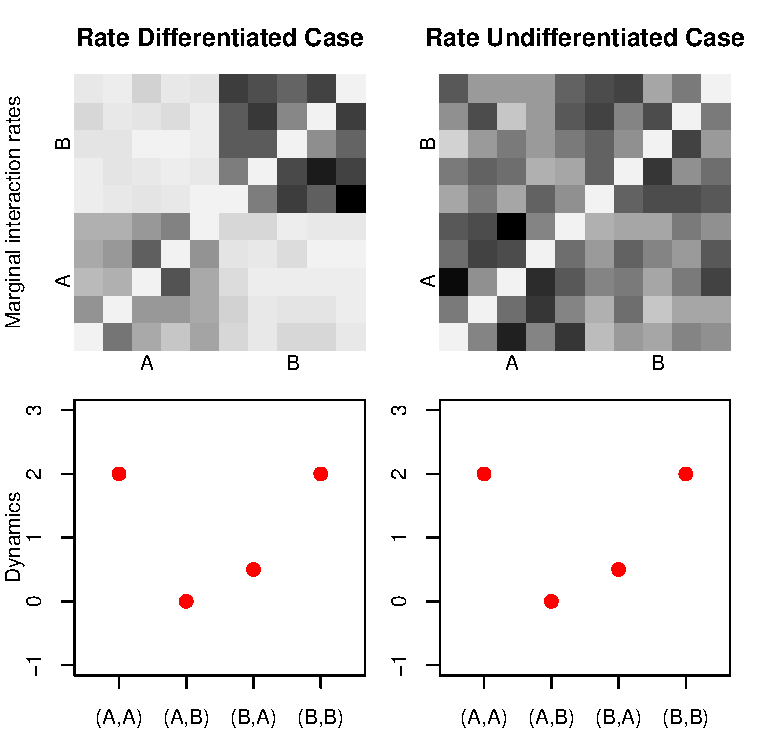
\includegraphics[scale=.45]{../figs/introexample/all}
\caption{Illustration of differentiation by rate of interaction versus by dynamic behavior.  The left column shows an example where within-block communication is large, and there is a higher tendency for reciprocity within a block.  In the situation where the two groups are not differentiated by rate, as in the right column, a standard blockmodel is unable to distinguish between groups A and B.  The proposed method can, however, learn such groups by employing more flexible definitions of shared dynamics.}
\label{fig:introexample}
\end{SCfigure}
% {\color{red} (Suggest renaming "Dynamics parameters" to "Behavioral parameters" or something.  "Dynamics parameters" is not gramatically sound.)
